%!TEX root = ./template-skripsi.tex
\addcontentsline{toc}{chapter}{LAMPIRAN}
\addtocontents{toc}{\protect\setcounter{tocdepth}{-1}}
\appendix
\chapter{Analisis Kebutuhan (\textit{User Requirement})}
\begin{figure}[H]
	\centering
	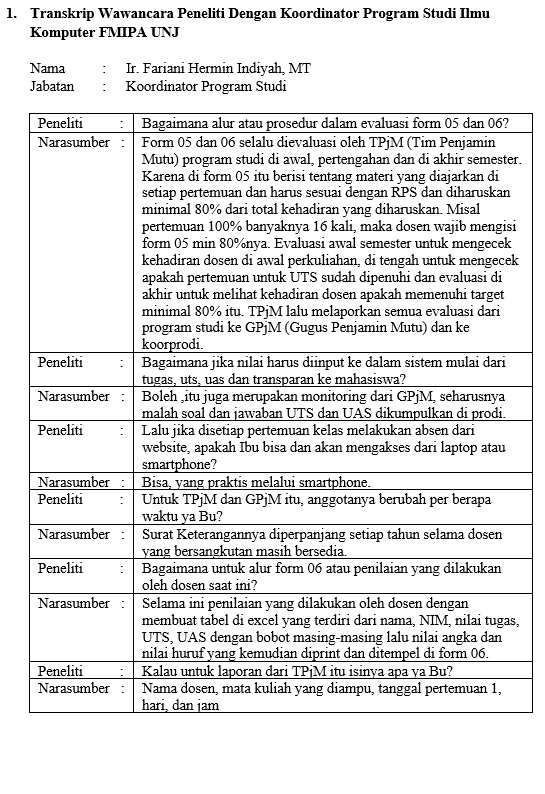
\includegraphics[width=0.9\textwidth]{gambar/lampiran/UR-1}	
\end{figure}
\begin{figure}[H]
	\centering
	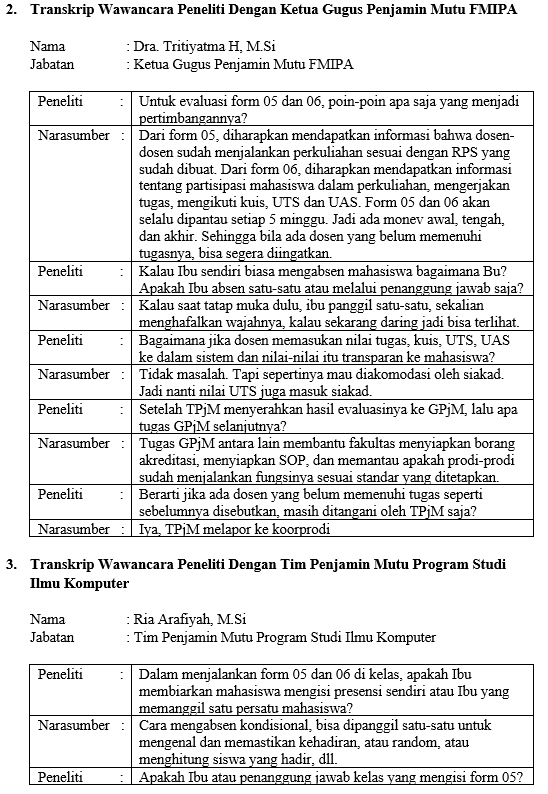
\includegraphics[width=0.9\textwidth]{gambar/lampiran/UR-2}	
\end{figure}
\begin{figure}[H]
	\centering
	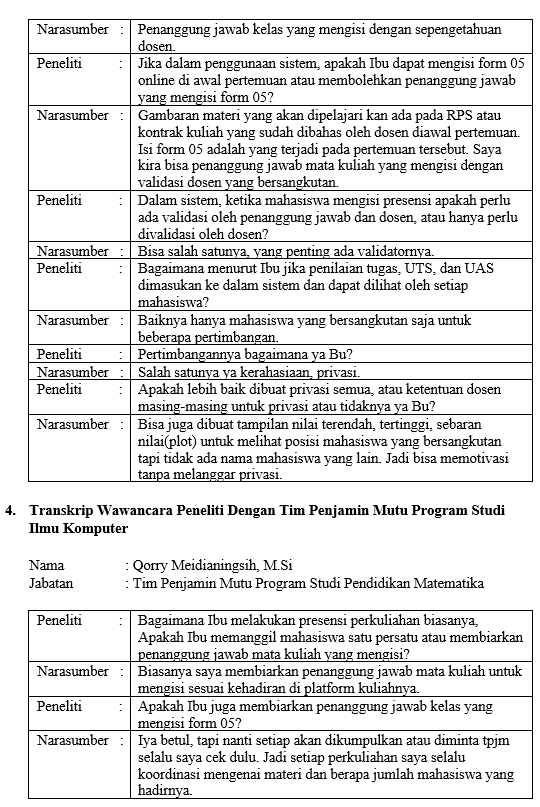
\includegraphics[width=0.9\textwidth]{gambar/lampiran/UR-3}	
\end{figure}
\begin{figure}[H]
	\centering
	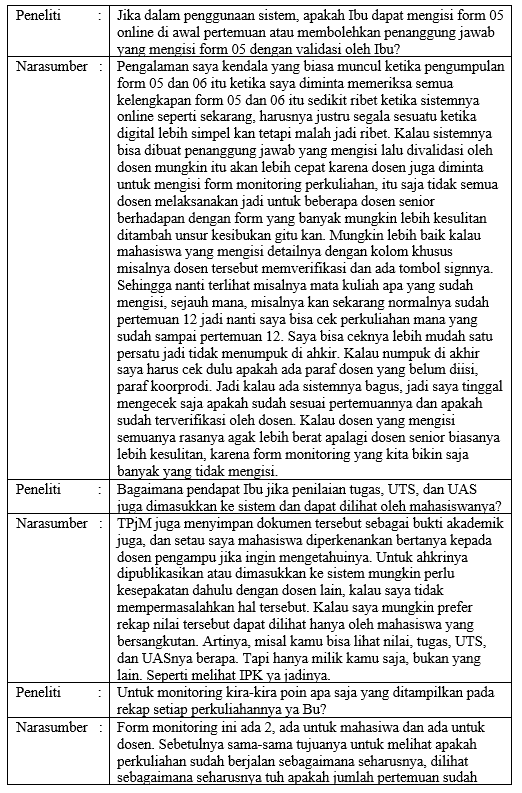
\includegraphics[width=0.9\textwidth]{gambar/lampiran/UR-4}	
\end{figure}

\begin{figure}[H]
	\centering
	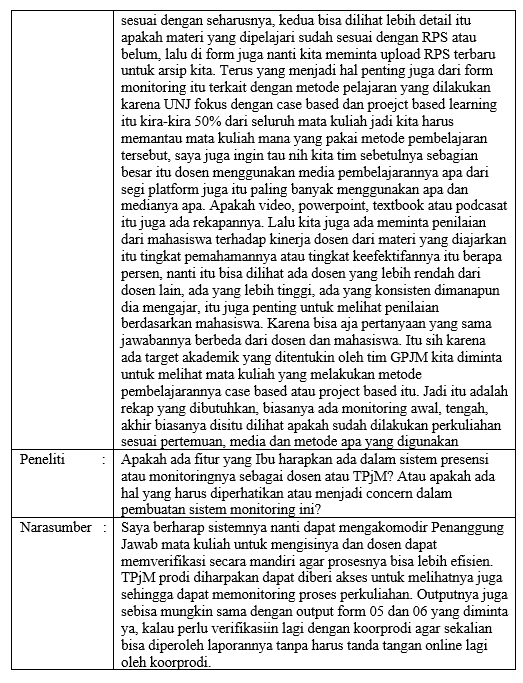
\includegraphics[width=0.9\textwidth]{gambar/lampiran/UR-5}	
\end{figure}

\chapter{Wawancara dengan Kepala UPT TIK}

\begin{figure}[H]
	\centering
	\includegraphics[width=0.9\textwidth]{gambar/lampiran/Wawancara Upt TIK}	
\end{figure}
